%%%%%%%%%%%%%%%%%%%%%%%%%%%%%%%%%%%%%%%%%%%%%%%%%%%%%%%%%%%%%%%%%%%%%%%%
%                                                                      %
%     File: Thesis_Background.tex                                      %
%     Tex Master: Thesis.tex                                           %
%                                                                      %
%     Author: Andre C. Marta                                           %
%     Last modified :  2 Jul 2015                                      %
%                                                                      %
%%%%%%%%%%%%%%%%%%%%%%%%%%%%%%%%%%%%%%%%%%%%%%%%%%%%%%%%%%%%%%%%%%%%%%%%

\chapter{Background}
\label{chapter:background}

%%%%%%%%%%%%%%%%%%%%%%%%%%%%%%%%%%%%%%%%%%%%%%%%%%%%%%%%%%%%%%%%%%%%%%%%
\section{Ray-Tracing}
\label{section:background_ray_tracing}

Ray-tracing \cite{Whitted80} is a global illumination \cite{Ritschel12} technique that is used for the synthesis of realistic images which employs recursive ray-casting \cite{Appel68}.

\medskip

The ray tracing algorithm casts primary rays from the eye but does not stop there. 
When the rays intersect geometry they can generate extra secondary rays: e.g. shadow, reflection and refraction rays.

\begin{figure}[!htb]
    \centering
    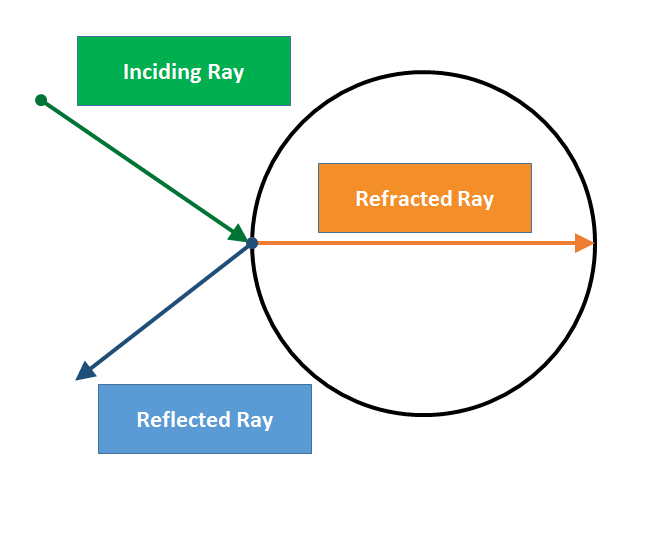
\includegraphics[scale=0.65]{Images/Secondary_Rays}
    \caption{\label{fig:bscr}Secondary Rays}
\end{figure}

These rays differentiate ray-tracing from the more traditional rasterization algorithm since they naturally allow realistic and complex effects like reflections, refractions and shadows without any need for additional techniques. However this comes with at price. Ray-tracing is computationally expensive. There is extensive research and ongoing to try and optimize it. Much of this research involves creating hierarchies in either the Object or Spatial domains to decrease the number of intersection tests in a divide and conquer fashion.

\medskip

Object and Spatial Hierarchies (like Octrees and Bounding Volume Hierarchies) help reduce the amount of intersections by reducing the amount of scene geometry required to test by culling many polygons and objects away from the ray paths at once (see Figure~\ref{fig:octree} and Figure~\ref{fig:bvh}).

\begin{figure}[!htb]
    \begin{minipage}{0.475\linewidth}
        \centering
        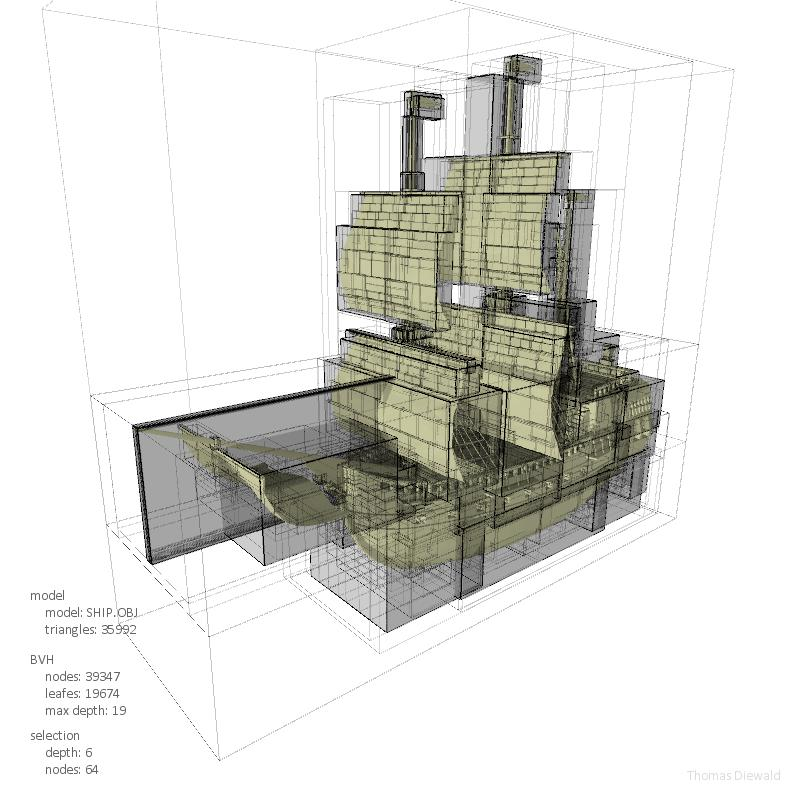
\includegraphics[width=6.0cm]{Images/BVH_Render}
        \captionof{figure}{\label{fig:octree}Octree}
    \end{minipage}
    \begin{minipage}{0.475\linewidth}
        \centering
        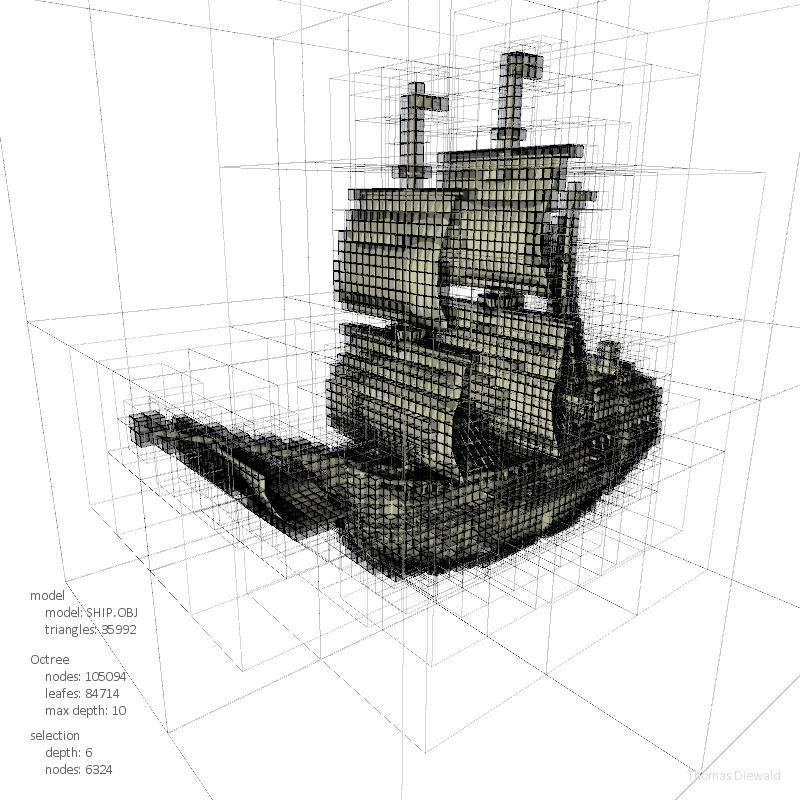
\includegraphics[width=6.0cm]{Images/Octree_Render}
        \captionof{figure}{\label{fig:bvh}Bounding Volume Hierarchy}    
    \end{minipage}
\end{figure}

Ray-Space Hierarchies, use ray bundles or ray caching mechanisms to achieve the same goal, reduce the number of intersections. Instead of creating hierarchies based on the scenes geometry, they are based on the rays being cast in each frame. This is the approach we decided to take is based on ray bundling but also uses a feature of ray caching, which is ray hashing \cite{Arvo87} \cite{Aila10}.

\begin{figure}[!htb]
    \begin{minipage}{0.475\linewidth}
        \centering
        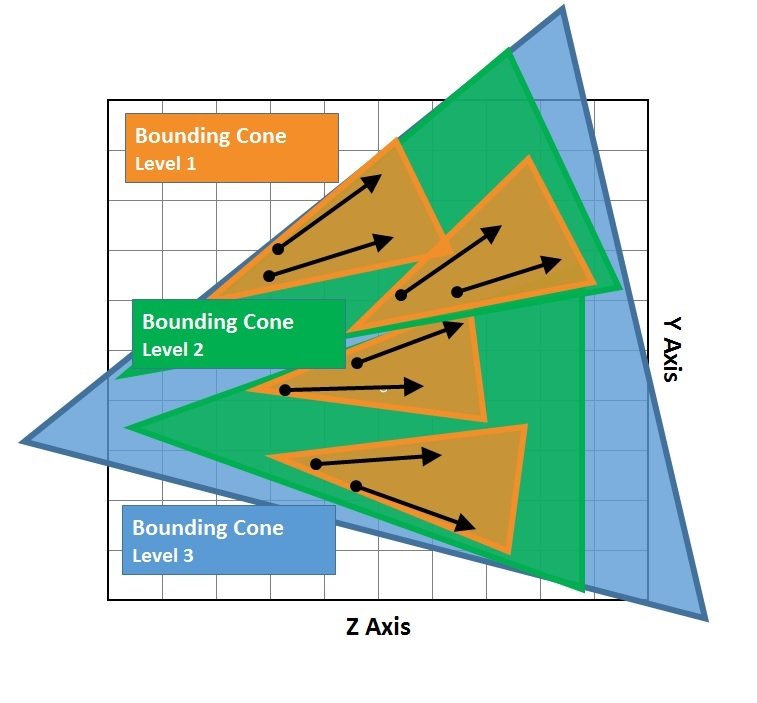
\includegraphics[width=6.0cm]{Images/Bounding_Cone}
        \captionof{figure}{\label{fig:bbc}Bounding Cone}
    \end{minipage}
    \begin{minipage}{0.475\linewidth}
        \centering
        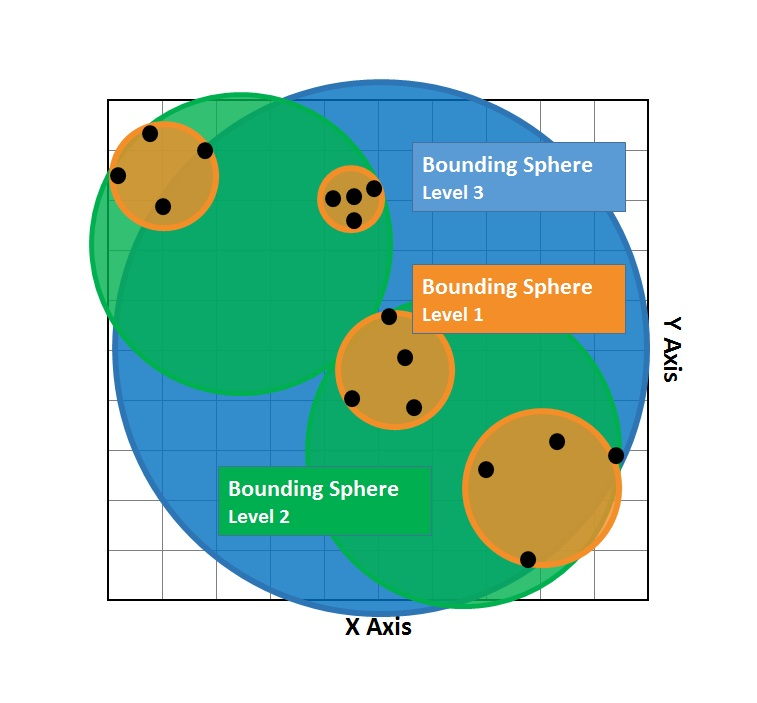
\includegraphics[width=6.0cm]{Images/Bounding_Sphere}
        \captionof{figure}{\label{fig:bbs}Bounding Sphere}    
    \end{minipage}
\end{figure}

\pagebreak

%%%%%%%%%%%%%%%%%%%%%%%%%%%%%%%%%%%%%%%%%%%%%%%%%%%%%%%%%%%%%%%%%%%%%%%%
\section{Fast Ray Tracing by Ray Classification}
\label{section:backgroud_arvo97}

Arvo and Kirk \cite{Arvo87} introduced a 5-dimensional ray-space hierarchy. They subdivided the ray-space in such a way that all relevant rays are distributed among equivalence classes. These classes are associated with a candidate object set. For example, the candidate set C\textsubscript{i} contains the objects that the rays in the equivalence class E\textsubscript{i} can intersect. The focus of this algorithm is to decrease the number of intersection tests.

\medskip

Since this algorithm works in a 5-dimensional space, the first thing we need to know is which are the degrees of freedom that a ray actually has. Traditionally rays are represented by a point and a vector in a 3-dimensional space, representing its origin and its direction. However a ray only has 5 degrees of freedom. These 5 degrees are its origin, which accounts for 3 degrees, and its direction, which accounts for 2 degrees when using spherical coordinates. This allowed Arvo and Kirk to parametrize rays and thus create subsets of the rays 5-dimensional space in such a way that rays with similar origins and directions would be in the same subset. 

\medskip

The algorithm was broken into 5 steps that I will now describe. It is also important to note that the first step is only carried out once while the second and third steps are consistently carried out in order to refine the hierarchy.

\subsubsection{1. Bounding Volume Creation}

The first step is to find the 5-dimensional bounding volume that contains the equivalent of each ray that can interact with the environment in said space. Since it's important to use volumes that don't take up too much space they chose to store 5 ordered pairs that represent intervals in the 5 orthogonal axes, which they labeled x,y,z,u and v. These 5 ordered pairs represent a bounding volume. Each of these bounding volumes, denominated hypercubes, have a representation in 3-dimensional space which they call a beam. This is vital to the algorithm because this beam comprises the points in 3-dimensional space that the set of rays contained in the hypercube can reach. One of the issues however is that the beams associated with the hypercubes are not generally polyhedra. To account for this fact, they used 6 different mappings that have the desired properties locally and together contain the whole ray-space. Each of the 6 mappings correspond to a dominant axis, x+,x-,y+,y-,z+ or z-, and one sixth of the direction space. The bounding volume is then created by creating six copies of the bounding volume created from the bounding box containing all the geometry. The rays are then mapped onto these bounding volumes.

\subsubsection{2. Space Subdivision}

The second step is to subdivide the 5-dimensional space into equivalence classes. The smaller each hypercube is, the more likely rays are to behave coherently. However, the smaller each hypercube is, the more classes we will have. The goal is to have hypercubes sufficiently small so that the rays of the corresponding beams intersect approximately the same objects, allowing the rays in that beam to share a set of candidate objects. Starting with the 6 bounding volumes created earlier, the hierarchy is created by subdividing each hypercube in half at each level, cycling each of the 5 axis. This continues until either the hypercubes size or the sets number of candidate objects fall below a fixed threshold. It is important to note that hypercubes are only subdivided if they contain rays generated during the ray-tracing process.

\subsubsection{3. Candidate set Creation}

For the third step each objects bounding box is intersected with the beam associated with the hypercube being tested. If there is an intersection then the object is added to that hypercubes candidate set. As the space is subdivided the candidate sets for the child hypercubes must be updated. Since there is an overlap between parent and child hypercubes they found that re-evaluating the candidate sets should only be done only after the hypercubes have been divided on all of the 5 axis, meaning a re-evaluation only after 5 subdivisions have occurred.

\subsubsection{4. Ray Classification}

The fourth step consists of finding the 5-dimensional hypercube that each ray corresponds to. This is done by mapping the ray to the 5-dimensional space and then traversing the ray-space hierarchy, beginning with the hypercube that is indexed by the rays dominant axis (this hypercube is one of the 6 copies created at the start of the algorithm) until the leaf containing the ray is reached. If the candidate set corresponding to this leaf is empty then the ray intersects nothing. Otherwise, we proceed to the next step.

\subsubsection{5. Intersection Tests}	

Finally the ray is tested with each object for intersections. Initially a coarse intersection test is carried out by using the objects bounding volume instead of the actual object, in order to reject rays that don't intersect the object.

\subsection{Considerations}

This algorithm works similarly to a Hash Tree, in the sense that each ray is converted to a key (in this case the corresponding 5-dimensional point) and after finding out which class it belong to (the classes can be associated with the equivalence classes) it is then mapped to a value (in this case the candidate object set). For dynamic scenes it would be necessary to recalculate the candidate sets each time the objects moved, which would be very costly. This means that the ray-space hierarchy is tightly connected to the objects and their positioning in the scene. This suggests that the algorithm is not a very good fit for ray-tracing of dynamic scenes, which is my goal. The ray caching scheme is interesting however if used differently, i.e. for the sorting of secondary rays.

\vfill

%%%%%%%%%%%%%%%%%%%%%%%%%%%%%%%%%%%%%%%%%%%%%%%%%%%%%%%%%%%%%%%%%%%%%%%%
\section{Five-dimensional Adaptive Subdivision for Ray Tracing}
\label{section:backgroud_simiakakis94}

Simiakakis and Day \cite{Simiakakis94} introduced some improvements to Arvo and Kirks work \cite{Arvo87}. These improvements consist of using a directional subdivision method, which adapts automatically according to the scene. They also introduced a memory saving scheme but the main issues with Arvo and Kirks paper with dynamic scenes still remain, which does not make this algorithm a good fit for dynamic scenes.

%%%%%%%%%%%%%%%%%%%%%%%%%%%%%%%%%%%%%%%%%%%%%%%%%%%%%%%%%%%%%%%%%%%%%%%%
\section{Whitted Ray-Tracing for Dynamic Scenes using a Ray-Space Hierarchy on the GPU}
\label{section:backgroud_roger07}

Roger et al. \cite{Roger07} presented an algorithm for interactive rendering of animated scenes with Whitted Ray-Tracing. This algorithm ran fully on the GPU and focuses on the secondary rays, using the GPU rasterizer to process the primary rays. They use a ray-space hierarchy that bundles rays together using cones and spheres. The algorithm is mapped on the GPU using textures to pass information between each of the algorithms phases.

\medskip

The algorithm consists of 5 steps that i will describe. It is important to keep in mind that the first step uses the GPU rasterizer since it has the same effect as tracing the primary rays but rasterizing them is faster.

\subsubsection{Render the Scene using the Rasterizer}

This step is done using the traditional rasterizer (for example using modern OpenGLs rasterization pipeline) that outputs the pixel color, without any kind of secondary ray effects like shadows,  reflections and refractions. Like it was stated  before, the primary rays give us the same pixel color as the standard rasterizer, so they took advantage of the performance of the rasterizer to speed-up the algorithm.

\subsubsection{Generate the first set of Secondary Rays}

Since fragment shaders can have multiple render targets, they take advantage of this fact to output the initial set of secondary rays as well. These rays can consist of the shadow rays, reflection rays and refraction rays.. Since the algorithm is generic enough, it does not matter which kind of secondary rays are used. It is also worth noting that the shadow rays are very coherent locally (if we're using soft shadows) so they fit cone hierarchy quite well.

\subsubsection{Build the Ray-Space Hierarchy}

The second step is taking the rays generated from the previous step and constructing the hierarchy. Each node consists of a structure composed by a sphere and a cone, which means that 8 floats are stored, 3 for spheres center and 1 for the spheres radius, 3 for the cones direction and 1 for the cones spread angle.i The hierarchy is constructed bottom-up, meaning that the leaves are constructed first. These leaves consist of spheres with radii 0 and cones with spread 0, representing the exact rays. The upper levels are then constructed by computing the union of the child nodes until we have a top node that encloses the whole ray-space.

\subsubsection{Intersect the Ray-Space Hierarchy with the Scene}

In this step the ray-space hierarchy is intersected with the scene. This is done in a top-down manner, testing each parent node before going down the hierarchy. Only triangles that intersect the parent node will be tested for intersections with the children nodes. This means that at each level of the hierarchy several triangles are removed from the intersection tests. It is also important to note that for this preliminary intersection phase the tests are carried out using the triangles bounding spheres since they are simply exclusion tests before the final local intersection tests. At each level of the hierarchy the intersection information is stored in textures, one for each of the 4 children nodes. If there is an intersection, the IDs for the triangle and the cone are stored in a texture, otherwise an empty element is stored. Since the texture will have blanks when there are failed intersection tests. These 4 textures also need pruned of empty elements  for the next pass.

\medskip

This has two purposes, one being memory management and the other being the mapping of the algorithm to the GPGPU. Since each pass stores its output in textures we can process each pass using the same operations meaning that there won't be threads having different execution paths which in turn is one of the features necessary to make an algorithm fit the GPU. These pruning methods are called stream-reduction passes and they presented two different methods, one involving an hierarchical version of Horns \cite{GPUGems2} and a slower one using geometry shaders. The hierarchical version works by breaking down the textures in components of fixed size and concatenating them at the end.

\subsubsection{Final Intersection Tests}	

Finally after traversing the hierarchy we have a texture with the triangle and  ray IDs (the last level of the hierarchy are individual rays), which means we need to calculate the traditional intersection tests, keeping the closest intersection.

\subsubsection{Considerations}

This algorithm works as a bounding volume hierarchy of sorts, adapted to the rays, using cones and spheres to enclose the ray bundles. It is also very well adapted to GPGPU since each pass has a fixed number of operations and has the same execution path. The stream-pass reduction method is vital since it helps prune the textures of empty elements, allowing the threads processing the textures to execute the same operations. Finally it leaves the possibility of combining the ray-space hierarchy with a object-space hierarchy, possibly reducing the number of intersections even more. It is also an example of hybrid rendering since it uses the GPUs rasterizer to compute the initial rays and the initial set of secondary rays.

\vfill

%%%%%%%%%%%%%%%%%%%%%%%%%%%%%%%%%%%%%%%%%%%%%%%%%%%%%%%%%%%%%%%%%%%%%%%%
\section{Fast Ray Sorting and Breadth-First Packet Traversal for GPU Ray Tracing}
\label{section:backgroud_garanzha10}

Garanzha and Loop \cite{Garanzha10} introduced an algorithm using various parallel primitives to adapt the ray-tracing algorithm to the GPU. Their algorithm sorts the generated rays and creates tight-fit frustums on the GPU and then intersects them with a Bounding Volume Hierarchy for the scenes geometry that is built on the CPU. One of the most interesting parts of their work is the fast ray sorting since it is done using parallel primitives which mitigates the overall cost of the operation when its executed on the GPU. I will now go into more detail regarding the four stages of the algorithm that they outlined.

\medskip

\subsubsection{Ray Sorting}

The first step, Ray Sorting, is used to store coherent rays in coherent memory locations in order to have less divergence during the tracing routine. If any given set of rays are coherent, they are more likely to intersect the same geometry and thus access the same memory locations. The sorting also allows the frustums in the next step to be tighter fits and thus give us a smaller set of intersection candidates.

\medskip

To sort the rays, they created a key-index pair for each ray, with the key being the rays ID and the index being the rays Hash value. This hash value is computed by quantizing the rays origin in a virtual grid that is within the scenes bounding box and then by quantizing its direction using a similar process.
After creating this pair for every ray, a compression-sorting-decompression scheme is used. This compression step generates chunks out of the initial set of rays. These chunks are represented by three arrays, the hash array (which indicates hash each chunk), the base array (which indicates the index of the first ray in each chunk) and a size array. This compression step takes advantage of the fact that it is likely that rays that are generated sequentially will have the same hash value. These chunks are then sorted using radix sort. The final step is the decompression, which applies an exclusive scan on the chunks size array to generate an array that indicates where each chunk will start in the re-ordered rays set.
After the exclusive scan two arrays are generated, the skeleton array that contains the base of the chunk in the positions from which the re-ordered rays set will be created from and the head flags array that indicates where new chunks start. An inclusive segment scan is then applied to these two arrays and the final re-ordered ray set is built. The final part of the decompression step is extracting the ranges of the packets of coherent rays. This is done by compressing the re-ordered ray set, using the same procedure that was used for the un-ordered ray set and then dividing those compressed chunks into packets, with a maximum size that is defined manually and then by decompressing using an inclusive segmented scan once more.

\subsubsection{Frustum Creation}

The frustum creation step picks up where the sorting left off. From the packet ranges calculated in the previous step a frustum is created for each one, using a dominant axis and two axis aligned rectangles to represent them, bounding each ray in the packet.

\subsubsection{Frustum Traversal}

The frustums are then intersected with the scenes Bounding Volume Hierarchy that was created on the CPU. This binary BVH has arity eight and 2/3rds of the tree levels are eliminated and an Octo-BVH is created. After traversing the BVH in a breadth-first order, each frustum will have a list of leaves assigned to it, which contain the primitives that will be used in the next step.

\subsubsection{Local Intersection Tests}

Finally the leaves are iterated on and for each of the primitives that they contain, localized intersection tests are calculated.

\subsubsection{Considerations}

This algorithm does not create a global Ray-Space hierarchy that contains every single ray. Instead, smaller local Frustums are created, taking advantage of the Ray-Sorting step to make them tight-fits. This reduces the number of leaves that each frustum will have assigned to it after traversing the Bounding Volume Hierarchy, which in turn reduces the number of localized intersection tests. The Ray-Sorting step is very interesting as it uses parallel primitives such as segmented scans to maximize its effectiveness on the GPU. This approach can be merged with Roger et al's \cite{Roger07} algorithm in order to create a more efficient RSH.